\documentclass[tikz,border=5mm]{standalone}
\usepackage{tikz}
\usetikzlibrary{arrows.meta, positioning, shapes.geometric, calc, patterns}

% --- COLOR DEFINITIONS ---
\definecolor{Garnet}{HTML}{73000A}
\definecolor{CBlue}{HTML}{466A9F}
\definecolor{CDark}{HTML}{1F414D}
\definecolor{CGold}{HTML}{A49137}
\definecolor{CGrayLight}{HTML}{E5E5E5}
\definecolor{CGrayDark}{HTML}{555555}
\definecolor{CWhite}{HTML}{FFFFFF}

\begin{document}

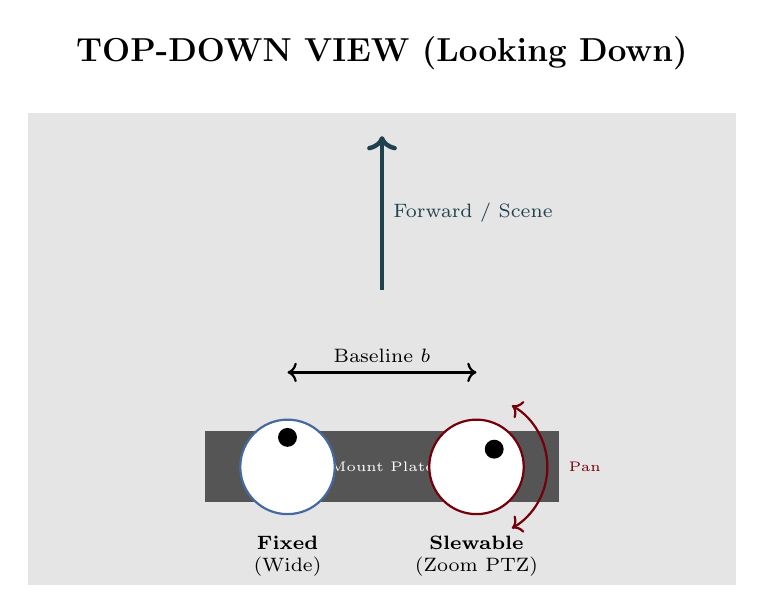
\begin{tikzpicture}[scale=1.5]
    % Title
    \node[font=\bfseries\large] at (0, 3.5) {TOP-DOWN VIEW (Looking Down)};
    
    % Ground / Floor reference
    \fill[CGrayLight] (-3, -1) rectangle (3, 3);
    
    % Tripod top plate (horizontal bar)
    \fill[CGrayDark] (-1.5, -0.3) rectangle (1.5, 0.3);
    \node[white, font=\tiny] at (0, 0) {Mount Plate};
    
    % Camera 1 (Left) - FIXED
    \fill[CWhite] (-0.8, 0) circle (0.4);
    \draw[CBlue, thick] (-0.8, 0) circle (0.4);
    \fill[black] (-0.8, 0.25) circle (0.08); % Lens pointing "up" in this view = forward
    \node[below, font=\scriptsize, align=center] at (-0.8, -0.5) {\textbf{Fixed}\\(Wide)};
    
    % Camera 2 (Right) - SLEWABLE PTZ
    \fill[CWhite] (0.8, 0) circle (0.4);
    \draw[Garnet, thick] (0.8, 0) circle (0.4);
    \fill[black] (0.95, 0.15) circle (0.08); % Lens pointing at angle
    \node[below, font=\scriptsize, align=center] at (0.8, -0.5) {\textbf{Slewable}\\(Zoom PTZ)};
    
    % Pan arrows for PTZ
    \draw[->, Garnet, thick] (1.4, 0) arc (0:60:0.6);
    \draw[->, Garnet, thick] (1.4, 0) arc (0:-60:0.6);
    \node[right, font=\tiny, Garnet] at (1.5, 0) {Pan};
    
    % Baseline distance
    \draw[<->, thick] (-0.8, 0.8) -- (0.8, 0.8) node[midway, above, font=\scriptsize] {Baseline $b$};
    
    % Forward direction arrow
    \draw[->, ultra thick, CDark] (0, 1.5) -- (0, 2.8) node[midway, right, font=\scriptsize] {Forward / Scene};
    
\end{tikzpicture}

\end{document}
